\documentclass[runningheads,a4paper]{./llncs2e/llncs}
\usepackage{graphicx}
\usepackage{fixltx2e}
\usepackage{mathtools}
\usepackage[nolist,nohyperlinks]{acronym}
% Maintain images and tables within their respective sections
\usepackage[section]{placeins}

%used in introduction in code
\usepackage{listings}
\usepackage[table]{xcolor}% http://ctan.org/pkg/xcolor
% 
% Change the margins
% 
% \usepackage[margin=2.9cm]{geometry}
%\author{Rafael Reia  and Ant\'{o}nio Menezes Leitão}

\begin{document}
\title{Refactoring for Dynamic Languages}

%\subtitle{Your Thesis subtitle}
\author{Rafael Reia,rafael.reia@tecnico.ulisboa.pt}
\authorrunning{Rafael Reia}
\titlerunning{Refactoring for Dynamic Languages}
\institute{Instituto Superior T\'ecnico, Universidade de Lisboa}

\maketitle

%!TEX root = ../report.tex

% 
% Abstract 
% 

\begin{abstract}
Dynamic languages are becoming popular, specially among unexperienced programmers, and the need for refactoring tools for dynamic languages is increasing.
Static language such as Java have several refactoring tools, however, there is a lack of refactoring tools for dynamic languages.
This paper present an overview of the refactoring tools for dynamic languages, such as Scheme, JavaScript, Smalltalk, Python and Racket.
It also proposes a refactoring tool for dynamic languages targeted for unexperienced users.

\end{abstract}
%!TEX root = ../report.tex

% 
% Keywords 
% 

\begin{keywords}
Refactoring tools, Dynamic languages, Static languages
\end{keywords}
%!TEX root = ../report.tex

% 
% Introduction
% 

\section{Introduction}


%Introduce the Refactoring Tools
Over time, software tends to change, new requirements appear or are adapted. 
Even after development new bugs are found or some critical new features are added.
%A piece of software that is used never stops changing and evolving.
This changes makes the software drift apart from its original design.
Typically these changes increase the complexity of the software, making it less readable and harder to change. 
Consequently, it makes the quality lower and the maintenance costs higher.
Continuous changes create the a need for continuously improving of the software structure.

Refactoring is a meaning-preserving transformation or a set of meaning-preserving transformations that are meant to improve the program structure and the software quality \cite{bourquin2007high}.
Thus, making refactoring a very desirable operation to maintain the software quality, but because it is a tedious and error prone activity it is preferable to use a tool that provides automated support. %to the refactoring operations that the programmer intends to do. 
Therefore saving time and preventing the addition of errors to a previous correct program.

%
%talk about the lack of refactoring tools for unexperienced users and maybe the importance of using refactoring tools while learning how to program.
Refactoring tools are important, however there is a lack of refactoring tools designed for unexperienced users.
They tend to create one big function that does all the program work and often use try and error to get the program correct.
This makes the program quality weak and needing a refactoring. 
By having refactoring operations available they could easily improve the program structure.
Because of the way unexperienced users usually program, by creating one big function, an important refactoring operation an unexperienced user would do besides the rename is the extract-method. 

By having a refactoring tool that allows the user to extract functions the unexperienced users would improve the quality of the program in a safe way.

%give the example
% Example extract method. Unexperienced users create one big function that do all the program work. Create a function that should clearly have a function extracted from the inside.
 Listing~\ref{lst:Fibonnacci} is an implementation of the Fibonacci function in Python and Listing~\ref{lst:FibonnacciRefactored} is an example of how a user would use the extract function refactoring operation.

\begin{lstlisting}[frame=single, caption=Fibonacci function first implementation, label={lst:Fibonnacci}, language=Python]
def fibonacci(number=1):
	previous = 0
	current = 1
	fib_numbers = []

	for i in range (0, number):
		aux = current + previous
		previous = current
		current = aux
		fib_numbers.append(current)

	for i in range(number):
		print fib_numbers[i]
\end{lstlisting}


\begin{lstlisting}[frame=single, caption=Fibonacci function after using extract function, label={lst:FibonnacciRefactored}, language=Python]
def fibonacci_seq(number):
	previous = 0
	current = 1
	fib_numbers = []
	for i in range (0, number):
		aux = current + previous
		previous = current
		current = aux
		fib_numbers.append(current)
	return fib_numbers

def print_fibonacci(fib_numbers, number):
	for i in range(number):
		print fib_numbers[i]

def fibonacci(number=1):
	fib_numbers = fibonacci_seq(number)
	print_fibonacci(fib_numbers, number)
\end{lstlisting}


In the refactoring, the user starts by choosing a set of expressions to extract, usually it is a  basic block or a set of basic blocks.
There are two functions extracted, the ``print\_fibonacci'' and ``'fibonacci\_seq''.
%talk about refactoring for static languages and dynamic languages

The use of the refactoring tools is fully adopted by the object oriented and static programming languages with their IDEs (integrated development environment) support.
For example, languages such as Java with the IDEs, Eclipse\footnote{https://eclipse.org/}, IntelliJ\footnote{https://www.jetbrains.com/idea/} or NetBeans\footnote{https://netbeans.org/} and C\# with Visual Studio\footnote{https://www.visualstudio.com/}.
%When compared to the dynamic languages there is a lack of refactoring tools and refactoring operations.
%talk about the lack of refactoring tools for dynamic languages
Unfortunately that is not the case for the refactoring tools for dynamic languages. 
The lack of information available during the refactoring about the program is the biggest difference between refactoring tools for static languages and refactoring tools for dynamic languages.
This difference is the main difficulty that made the refactoring tools for dynamic languages not evolve like the ones made for static languages. 
Therefore making the refactoring tools for static languages largely used and considered a common tool in contrast with the refactoring tools for dynamic languages.  %Does not sound good.

Nonetheless the importance of dynamic languages is growing. Dynamic languages are becoming popular among the scientific community.
In addition to that, dynamic languages are often used as a learning language in introductory courses around, for example, Scheme, Racket and Python.

%Conclude with the need of having such refactoring tool
A refactoring tool for a dynamic language concerned with unexperienced users would be an important step in filling the lack of refactoring tools for dynamic languages and it also would help the unexperienced users to have the first contact with refactoring tools and improve their code quality.


%say what will be addressed in the next sections.

The Section 2 addresses the objectives for this thesis work. 
Section 3 describes some definitions related to refactoring tools, such as the types of refactoring tools.
Section 4 describes how the users refactoring, it compares refactoring tools for static languages, it describes refactoring tools for dynamic languages, and it describes language-independent refactoring tools.
Section 5 describes the architecture of the proposed solution. 
Section 6 explains how the tool will be evaluated and finally section 7 sums up the work.






%[REF]evolution survey do ments.
%\cite{drscheme} teste  \cite{drscheme_pegadogy} \cite{languages_scheme}
%Over time, software artifacts tends to change, in order to develop gradually, to expand %quando se esta a usar, depois de se usar durante algum tempo
%while being used and even during development, new requirements appear, the existing ones change, new bugs are found or some critical %SHINY! important
%new features are added.

 %[REF] Case study in refactoring functional programs.&& [REF] Refactoring: current research and future trends.


%Preserving the meaning is important because if the meaning changes, it transforms the program in a different program.

%[REF] FIND IT 
%The difference between Refactoring and restructuring is that Refactoring is used in literature to define the transformations that improve the program preserving the behavior in Object Oriented paradigm \cite{opdyke1992refactoring} \cite{fowlerrefactoring1999} whereas Restructuring is used for the rest. \cite{griswold1993automated} \cite{softrest1986} %[REF] 


%why we need refactoring tools[ref JunGL]






%The purpose of this paper is to show which refactoring tools exist for dynamic languages. %change this.




%The Section 2 addresses the objectives for this thesis work. Section 3 explore related work in refactoring and restructuring programs, some implemented restructuring tools and some implementations of language independent refactoring tools. Section 4 describes the architecture of the proposed solution. Section 5 explains how the tool will be evaluated and we conclude on section 6.




%!TEX root = ../report.tex

% 
% Objectives
% 

\section{Objectives}

%The objectives of this thesis is to implement refactoring operations for inexperienced users.

%To do that it is important to have a language suited to beginners and a pedagogic IDE.

%Refactoring the program using refactoring tools is safer than manually, therefore it prevents introduction of bugs in a previous correct code.
%give example of rename, don not rename all the variables, there is some that are forgotten and stuff

%besides that when programming the inexperienced users tend to create a big function for everything and do not subdivide that function in smaller functions. (extract function refactoring)

The main goal of this thesis is to implement refactoring operations adequate for inexperienced users.
Because it is targeted for inexperienced users it is ideally designed for a language that is used to teach programming in introductory courses worldwide, for example Racket or Python.
It is also important to have a pedagogic environment instead of complex IDEs such as Eclipse.
Having a refactoring tool for inexperienced users is important because those users probably will not get the program right at first try.
Using a refactoring tool to do the refactoring operation will do a quicker and better job because it is safer than doing it manually.

Those operations must be:
\begin{itemize}
\item Correct
\item Simple to use
\item Useful
\end{itemize}

These characteristics are fundamental to create a refactoring tool targeted for inexperienced users.
%!TEX root = ../report.tex

\section{Definitions}


%add refferences

%[REF] Survey of software refactoring tools \cite{erb2010survey}
This section presents some definitions regarding refactoring activities.

\subsection{Classification of the refactoring}
There are several levels of refactoring, from a high-level refactoring, like design refactoring, to a low-level refactoring such as the extract method refactoring operation.
In between, exists combinational refactoring that is a combination of several low level refactoring operations.
Refactoring operations can also be classified by the effect they have on software quality attributes.
In order to classify the effect based on software quality attributes, it is necessary to map the changes in the internal software quality metrics, e.g. lines of code, cohesion or coupling, to the external software quality attributes, e.g. adaptability, reusability or testability. \cite{elish2011classification}
However, this is a complex task that is outside the scope of this thesis and therefore it will not be further detailed.

%(i) internal software quality metrics and (ii) external software quality attributes (adaptability, completeness, maintainability,
%understandability, reusability and testability). The classification is done by mapping the changes in the
%internal quality metrics, caused by applying refactoring methods, to the external quality attributes.

\subsection{Refactoring as a Process}
Refactoring can be done in two ways. %add citations
One is doing the refactoring in between programming and constantly performing it.
The other one is to do the refactoring as a separate activity and done in bulk.
Regardless when is done, the refactoring can always be decomposed in different activities: \cite{erb2010survey}

\begin{enumerate}
 \item Identify where to change the software
 \item Determine the adequate refactoring operation
 \item Have a way to protect the planned changes (e.g, automated tests)
 \item Make the planned changes
 \item Access the refactoring benefits
 \item Maintain consistency between refactored and non-refactored code
\end{enumerate}


%Eisenecker et al. [2000] defined requirements for the refactoring tools

%Functional requirements of a refactoring tools:
%Image, or explain in text => explain in text
%Non Functional requirements of a refactoring tool:
%Image. or explain in text.

\subsection{Refactoring Correctness}
%survey of software refactoring tools \cite{erb2010survey} %add citation
%
Refactoring must preserve the program's behavior in order to be correct.
However, there is no consensual definition for what behavior preservation is.
Some authors say that the behavior of the program is the output and preserving the input-output behavior preserves the program behavior suggested by Opdyke \cite{opdyke1992refactoring}.
However, other authors think that preserving the output is insufficient, since other aspects may be relevant as well. For example, for real-time software, the execution time of certain operations is an important aspect of the behavior.
One way to deal with behavior preservation is to have an extensive set of test cases and if all these tests still pass after the refactoring, it is highly probable that the refactoring is correct \cite{mens2004survey}.
A more formal approach is to prove that the refactoring operations preserve the full program semantics. For Prolog, that has simple and formally defined semantics, it is simple to prove that refactoring preserve the program semantics \cite{proietti1991semantics}. %27?
But for more complex languages such as C++, which the formal semantics is extremely difficult to define, typically it is necessary to put restrictions to the refactoring operations or to the language constructs and the refactoring tool may be limited to a particular version of a particular compiler \cite{tokuda2001evolving}.%28?
% \cite{mens2004survey}.

%For example in a class, if a method name is renamed and the program consists in printing that method name, by renaming that method the behavior of the program changes.

%Another way do define it is to say that in order to preserve behavior it is necessary to preserve the syntactically and semantic properties.
%Preserving the syntactic properties is to still have a well-formed program after the transformation, and it is common sense that a refactoring should not invalidate a syntactic correct program.

%Preserving the semantics of the program means to preserve the meaning of the program in the basic concept of the language.
%In other words, the semantic properties of all declarations after a refactoring should resolve to the same declarations they resolved before the transformation.
%Because preserving the syntax is easily seen, this document focus on the meaning-preservation of the refactoring operations.


%suvey mens 2003 \cite{mens2003refactoring}
%What is behaviour and how to preserve it?
%Observational behaviour, for the same input we get the same output, is not always sufficient.
%for example, for Real time systems it is important the time that a (sequence of) operations takes, for embedded systems it takes into account the memory and the power consumption and for safety-critical systems there is a defined safety that must be preserved.
%In a theoretical world all this properties should be preserved by a refactoring, however in practice that is not the case.

\subsection{Case Study - Manual Refactoring}

One way to learn how the users manually refactor is to do it while taking notes.
%The case study \cite{thompson2003case} was done with the idea to show that refactoring is also important in functional programs.
The case study \cite{thompson2003case} consists in refactoring an Haskell program with 400 lines, written by a student.
The program's goal is to build a semantic tableaux, which is a truth tree used for example to proof procedures for first order logic or solve satisfiability of finite sets.

%\subsubsection{Refactoring of a program}
In order to better understand in what consists a refactoring they applied manual refactoring operations to the program.
They started by changing the name of some variables to avoid misunderstandings and to be easier to read.
After that they renamed some functions to names that reflect better what the function did.
Then they replaced explicit recursion by calls to higher order functions and they rename some variables and functions.
In the end they generalized some functions and modified the representation type because it was giving a lot of work keeping the initial representation.

%\subsubsection{What was learned}
This case study shows that the order of the refactoring operations is somehow arbitrary.
The refactoring operations were applied whenever they thought it made more sense.
They also conclude that generally, refactoring a program is a good way to find out more about the program.
And that the refactoring operations need to have a way of doing undo, redo or revert changes, otherwise it would be more difficult to correct mistakes.

It is crucial to document the refactoring operations applied in detail.
This aspect was stressed because having documentation about the version previous to the refactoring, or outdated, is not good for the readability of the program since it can mislead the programmer.


\subsection{Classification of refactoring tools} %\cite{erb2010survey}
Refactoring tools can be subdivided in manual, semi-automated and fully-automa\-ted according to the degree of automation.
In the manual case there is no support for detecting refactoring opportunities, but the transformation is applied by the refactoring tool. If the transformation itself is left to the user, the tool can not be considered a refactoring tool.
The fully-automated one, automatically identifies refactoring opportunities and automatically applies them.
Finally the semi-automated one identifies refactoring opportunities but waits for the user to decide the application of the refactoring.



%\subsection{Levels of Refactoring}
%There are different kinds of refactoring.
%There is manual, that is refactoring without tool support.
%Syntactic, refactoring only focused on the syntax transformations.
%Semantic, the most common one, takes into account the syntactic and semantic information in the transformations.
%And finally there is the Automated, that automatically detects the possible refactoring operations to be applied.


% subsubsection subsubsection_name (end)

\subsubsection{Manual Refactoring Tool}
is a refactoring tool that applies the refactoring operations selected by the user.
Is available for all kind of languages and it is the most common level of refactoring.
%Besides that, and in contrast with the object oriented languages, there is a lack of semantic refactoring tools for dynamic languages.
There are several examples of this tools, including Eclipse and IntelliJ that are focused in static languages and for dynamic languages there is the refactoring browser for Smalltalk.
This kind of tools will be further detailed in the related work section.
%Semi-Automated Application   & The Refactoring Browser \cite{roberts1997refactoring}, Griswold \cite{griswold1993automated} \\ \hline
%\subsubsection{Syntactic refactorings}
%prof paper

%In this paper \cite{leitdo2002formal} it is proposed a pattern language refactoring tool that works well on lisp-like languages.

%The pattern is composed by transformations that are described in a simple syntax and even that the pattern is composed by operations of simple syntax they are composable, which makes it easier for the programmer to extend the refactoring tool, and there is no impediment to create complex transformations.

%The tool also can induce transformation rules based on manual examples given by the programmer and then if needed the programmer can easily extend those rules.

%This tool is simple because it is focused on syntax transformations of the program.
%Meaning that it does not need semantic information such as bindings relations needed for transformations, making it a simpler tool.


\subsubsection{Semi-Automated Refactoring Tool}
is a refactoring tool that suggests refactoring opportunities to the user and applies the refactoring operations that the user selected.
In order to know what refactoring operations to do, the tools can use metrics that can support the decision of where and which refactoring operations to apply.
The tool \cite{simon2001metrics} was created as proof of concept and it uses the metrics to identify where the code should be refactored.
The tool takes into account the "bad smell" of a code to suggest a refactoring.
A "bad smell" is a human intuition in which a specific code should be refactored.
An example of a ``bad smell'' that trigger a Move method refactoring, which moves a method from one location to another, occurs when one method is used more by other class than the class in which the method is defined.

%An example of a "bad smell" that would trigger a Move Method refactoring, that moves a method from one location to another, is when one method of a class is used more by other class in which it is defined.

To quickly show to the user the identified "bad smells" a visualization of the methods and attributes is generated and those objects are linked to the corresponding source code, as it can be seen in the Figure~\ref{fig:MetricsBasedRefactoring}.

\begin{figure}[h!]
  \centering
  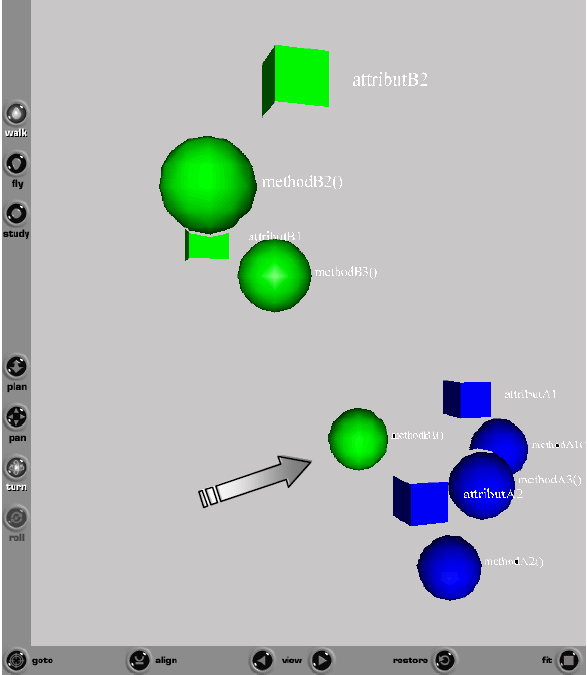
\includegraphics[width=0.75\textwidth]{img/metricsbasedrefactoring.png}
  \caption{Motivates the refactoring move method}
  \label{fig:MetricsBasedRefactoring}
\end{figure}

%\subsubsection{Distance based cohesion on refactoring operations}
In order to make an automated approach to identify "bad smells" a distance based cohesion metric is used.
With the distance based algorithm it is possible to identify violations to the rule "put together what belongs together".
There are some refactoring operations that are related to this rule such as, move attribute, extract class, in-line class and move method.
Regarding the distances, a method using only locally defined methods or attributes has a high distance to the methods of other classes, whereas methods that use many attributes and/or methods of other classes have a low distance to them.
The attributes are compared by the methods that use them.
For example if an attribute is only used by methods of other classes, that attribute probably should be moved to a different class.

\subsubsection{Automated Refactoring Tool}
is a refactoring tool that automatically applies the refactoring opportunities that the tool detects.
This kind of tool is useful when doing a source to source transformation, eliminating features that are not necessary and translating them into equivalent ones.
For example, if there is a profiling tool that only works in the previous versions of Java 1.4 and the user wants to use such profiling tool, an automated refactoring tool can be used in order to refactor the program by translating the new features, such as anonymous classes, into equivalent ones.
However, automated refactoring tools can also be used like a normal refactoring tool but has some restrictions because the user do not know what the refactoring tool is doing.
Casais \cite{casais1994automatic} or Moore \cite{moore1996automatic} are good examples of those refactoring tools.

%finding common attributes of classes and pulling those up into new super-classes
%GURU is a fully automated  tool for refactoring inheritance hierarchies and refactoring methods in SELF programs

%refactoring automaticas, source to source, e alinguagem source tem features que nao quero tratar. e elimina essa features, eg traducao pos 1.4 to pre 1.4 classes internas anonimas. ferramenta so funciona com versao antiga eg profiling.
%Automated                    & Casais \cite{casais1994automatic} or Moore \cite{moore1996automatic}

%The automated ones are used to improve internal software quality by removing the duplication of methods and attributes. However this tools have problems in preserving the understandability.
%There is no current or little practical relevance for full-automated approaches.


\subsubsection{Analysis:}
Having the automated refactoring tool for inexperienced users is not what is intended.
Transforming automatically the program will create a new program that the user might not comprehend, especially if the user is inexperienced.

The Semi-automated tool with the suggestions would be an advantage to inexperienced users that are still learning what refactoring operations exists and that way the users would learn new refactoring operations and have programs with better quality.
However, detecting refactoring opportunities is highly dependent on the application domain, witch invalidates this type of tools since they are not meant for one type of application only.

The ideal approach is a Manual Refactoring tool that applies exactly what the user wants to do.
This type of tool do not automatically detects refactoring opportunities, but it is faster and safer than doing the refactoring operation without any support.

%!TEX root = ../report.tex

% 
% Related work
% 

\section{Related Work}


This section starts to present the use of refactoring tools and an overview of static refactoring tools.
After that it presents the refactoring tools for the dynamic languages such as, Scheme, JavaScript, Smalltalk, Python and Racket.
Then it presents the language-independent refactorings.
Finally it has a conclusion about the related work.

%How we Refactor, and how we know it.
\subsection{Use of static refactoring tools}

Understanding how users refactor and use refactoring tools is an important step to better improve the later.
The information necessary to reason about how the users refactor was gathered by collecting some data sets \cite{murphy2012we}.


%Murphy et al \cite{murphy2012we} collected some data sets in order to understand how the users refactor.
The User data set was collected \cite{murphy2006java} in 2005, it has records of 41 volunteer programmers using eclipse, from which, 95\% of them programmed in Java. %Whit this we implied that Refactoring tools are underused [10]

The Everyone data set was collected from the Eclipse Usage Collector, the data used aggregates activity from over 13000 Java developers between April 2008 to January 2009 and it also includes non-Java developers.

The Toolsmiths data set that consists in information about 4 developers who primarily maintain eclipse's refactoring tools from December 2005 to August 2007. 
However, it is not publicly available and it is not described in other papers.
There is only a similar study \cite{robbes2007mining} that uses data from the author and another developer. 


%Many other authors have mined software repositories automatically for refactorings (WeiBgerber and Diehl [18]) they did not know of other research that compares refactoring tool logs with code histories.
Using all the data sets it is possible to see which are the most common refactoring operations used by the users and they are: rename, extract local variable, inline, extract method and move. The sum of the use percentages of this refactoring operations is between 86.4\% and 92\% of the data sets. % 86.4 90.8 92.0 

However the refactoring behavior differs among users. The most used refactoring operations is the rename for all the sets, but the used percentage drastically differs between Toolsmiths and the other sets. Toolsmiths usage of the rename refactoring is 29\% while the User set and Everyone set is 62\% and 75\% respectively.

Using the data sets of Users and Toolsmiths it was possible to confirm that refactoring operations are frequent. 
In the Users data set, 41\% of programming sessions contained refactoring activities and the sessions that did not have refactoring activities were the sessions where less edits were made.
In the toolsmith data set only 2 weeks of the year 2006 did not have any refactoring operation and, in average, had 30 refactoring operations per week. 
In 2007 every week had refactoring activities and the average was 47 refactoring operations a week.

Besides refactoring operations being frequent, the refactoring tools are underused. 
%In order to decide whether the refactoring operation was manual or tool assisted they tried to correlate refactoring activities with tool support. 
%If the refactoring activities is correlated with tool support it is classified as being a tool assisted refactoring.
After evaluating the refactoring activities in the data set they were unable to link 73\% of the refactoring operations to a tool supported refactoring. 
All this numbers are computed from the Toolsmiths data set which is in theory the group who knows, and better uses the refactoring tools.


\subsection{Overview of static Refactoring tools}
%\textbackslash
\begin{table}
\caption{Refactoring operations available by default}
\label{tab-Comparing-Static}
\begin{tabular}{|l|c|c|c|c|c|c|}
\hline\noalign{\smallskip}
Refactoring \textbackslash IDE           & Visual Studio & Eclipse & CDT & IntelliJ & NetBeans & Jbuilder \\
\noalign{\smallskip}
\hline
\noalign{\smallskip}
Rename                    & x             & x       & x   & x        & x        & x        \\ \hline
Move                      &               & x       & x   & x        & x        & x        \\ \hline
Change method signature   &               & x       &     & x        &          &          \\ \hline
Extract method            & x             & x       & x   & x        &          & x        \\ \hline
Extract local variable    &               & x       &     & x        &          & x        \\ \hline
Extract constant          &               & x       & x   & x        &          &          \\ \hline
Inline                    &               & x       &     & x        & x        &          \\ \hline
To nested 			      &               & x       &     & x        &          &          \\ \hline
Move type to new file     &               & x       &     & x        &          &          \\ \hline
Variable to field         &               & x       &     & x        &          &          \\ \hline
Extract superclass        &               & x       & x   & x        & x        &          \\ \hline
Extract interface         & x             & x       &     & x        & x        &          \\ \hline
Change to supertype 	  &               & x       &     &          & x        &          \\ \hline
Push down                 &               & x       &     & x        & x        &          \\ \hline
Pull up                   &               & x       &     & x        & x        &          \\ \hline
Extract class             &               & x       &     & x        &          &          \\ \hline
Introduce parameter       &               & x       &     & x        & x        &          \\ \hline
Introduce indirection     &               & x       &     &          &          &          \\ \hline
Introduce factory         &               & x       &     & x        & x        &          \\ \hline
Encapsulate field         & x             & x       &     & x        &          &          \\ \hline
Generalize declared type  &               & x       &     &          &          &          \\ \hline
Type Migration            &               &         &     & x        &          &          \\ \hline
Remove Middleman          &               &         &     & x        &          &          \\ \hline
Wrap Return Value         &               &         &     & x        &          &          \\ \hline
Safe Delete               &               &         &     & x        & x        &          \\ \hline
Replace Method duplicates &               &         &     & x        &          &          \\ \hline
Static to instance method &               &         &     & x        &          &          \\ \hline
Make Method Static        &               &         &     & x        &          &          \\ \hline
Change to interface 	  &               &         &     & x        &          &          \\ \hline
Inheritance to delegation &               &         &     & x        &          &          \\ \hline
\end{tabular}
\end{table}
 
\begin{table}[htbp]
\caption{Refactoring operations definitions:}
\label{tab-Refactoring-Definitions}
\begin{tabular}{ p{2.95cm}| p{9.15cm}}
\hline\noalign{\smallskip}
Refactoring name 		  & Definition \\
\noalign{\smallskip}
\hline
\noalign{\smallskip}
Rename                    & Renames the selected element and corrects all references.                                                                                                                 \\ \hline
Move                      & Moves the selected elements and corrects all references.                                                                                                                  \\ \hline
Change signature          & Change parameter names, types and updates all references.                                                                                                                 \\ \hline
Extract method            & Creates a new method with the statements or expression selected and replaces it with a reference to the new method.                                                          \\ \hline
Extract local variable    & Creates a new variable assigned to the expression selected and replaces it with a reference to the new variable.                                                             \\ \hline
Extract constant          & Creates a static final field from the selected expression.                                                                                                                \\ \hline
Inline                    & Inline local variables, methods or constants.                                                                                                                             \\ \hline
To nested                 & Converts an anonymous inner class to a member class.                                                                                                                      \\ \hline
Move type to new file     & Creates a new compilation unit and updates all references.                                                                                                                \\ \hline
Variable to field         & Turns a local variable into a field.                                                                                                                                       \\ \hline
Extract superclass        & Creates a new abstract class, changes the current class to extend the new class and moves the selected methods and fields to the new class.                               \\ \hline
Extract interface         & Creates a new interface and makes the class implement it.                                                                                                                 \\ \hline
Change to Supertype       & Replaces, where it is possible, all occurrences of a type with one of its supertypes.                                                                                     \\ \hline
Push down                 & Moves a set of methods and fields from a class to its subclasses.                                                                                                         \\ \hline
Pull up                   & Moves a field or method to a superclass, if it is a method, declares the method as abstract in the superclass.                                                            \\ \hline
Extract class             & Replaces a set of fields with new container object.                                                                                                                       \\ \hline
Introduce parameter       & Replaces an expression with a reference to a new method parameter and updates all callers of the method.                                                                  \\ \hline
Introduce indirection     & Creates an indirection method delegating to the selected method.                                                                                                          \\ \hline
Introduce factory         & Creates a new factory method, which calls a selected constructor and returns the created object.                                                                          \\ \hline
Encapsulate field         & Replaces all references to a field with getter and setter methods.                                                                                                        \\ \hline
Generalize type           & Allows the user to choose a supertype of the selected reference.                                                                                                          \\ \hline
Type Migration            & Change a member type and data flow dependent type entries.                                                                                                                \\ \hline
Remove Middleman          & Replaces all calls to delegating methods with the equivalent calls.                                                                                                       \\ \hline
Wrap Return Value         & Creates a wrapper class that includes the current return value.                                                                                                           \\ \hline
Safe Delete               & Finds all the usages or, simply delete if no usages found.                                                                                                                \\ \hline
Replace duplicates        & Finds all the places in the current file where the selected method code is fully repeated and change to corresponding method calls.                                      \\ \hline
Static to instance        & Converts a static method into an instance method with an initial method call argument being a prototype of newly created instance method call qualifier.                  \\ \hline
Make Method Static        & Converts a non-static method into a static one.                                                                                                                           \\ \hline
Change to Interface       & Used after using Extract an Interface it searches for all places where the interface can be used instead of the original class.                                             \\ \hline
Inheritance to delegation & Delegates the execution of specified methods derived from the base class/interface to an instance of the ancestor class or an inner class implementing the same interface. \\ \hline
\end{tabular}
\end{table}
%Por C++ e comparar ve o que o eclipse tem.
The {\bf table.~\ref{tab-Comparing-Static}} compares refactoring tools with each other and the Refactoring definitions, that were taken from Eclipse\footnote{help.eclipse.org/luna/topic/org.eclipse.jdt.doc.user/reference/ref-menu-refactor.htm} and IntelliJ\footnote{https://www.jetbrains.com/idea/features/refactoring.html} can be found on the {\bf table.~\ref{tab-Refactoring-Definitions}}.

The {\bf table.~\ref{tab-Comparing-Static}} compares the Visual Studio refactoring operations for C\# with Refactoring tools that have refactoring operations for Java because the languages are similar. It also compares with the Eclipse CDT  refactoring operations for C++ because in some aspects the languages are also similar and the refactoring operations compared are similar to the refactoring operations for Java or C\#. 
The table only lists the refactoring operations that each IDE has by default in order to have a fairer way to compare them with each other.
It is easy to see that IntelliJ has almost all the refactoring operations in this table, followed by Eclipse and NetBeans.
However, even having significantly less refactoring operations available by default than the other tools, JBuilder has the most used ones as shown above.
Visual Studio has only 2 out of the 5 most used refactoring operations available by default, but there are easily installed plug-ins that cover the more important refactoring operations. 

%It is easy to see all the effort to provide to the programmers refactoring operations to help them refactoring their projects. 


\subsection{Haskell}

HaRe \cite{thompson2005refactoring} is a refactoring tool for Haskell that integrates with Emacs and Vim.
This tool was made for being used instead of being a proof of concept prototype and it is implemented in Haskell.
The system also allows the users to design their own refactoring operations using the HaRe API.

The HaRe system uses an AST of the program to be refactored in order to reason about the transformations to do.
The system has also a token stream in order to preserve the comments and the program layout by keeping information about the source code location and the comments of all tokens.

%\subsubsection{Stages of Refactoring}
%\hfill \break

%{\bf Information gathering and condition checking:} The Refactoring will only be performed if it preserves the semantics of the program.
%It is needed some information, such as a set of identifiers of the scope, that information is gathered trough transversing the AST.

%{\bf Transformation:} After the conditions are verified, it is possible to apply the refactoring operation, which is a transformation of the AST.

%{\bf Program rendering:} After the refactoring operation the source code of the new program needs to be generated, keeping the original program layout as much as possible.

%insert pic?
%\begin{figure}[h!]
%  \centering
%  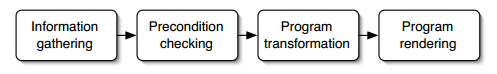
\includegraphics[width=0.75\textwidth]{img/HaReStagesOfRefactoring.png}
%  \caption{Stages of Refactoring}
%  \label{fig:HaReStages}
%\end{figure}
%add structural refactorings, module-aware? 

%\subsubsection{Refactorings Available} %review and change title
%\hfill \break

%Initially the HaRe system only had structural refactorings. 
%Structural refactorings care about the objects defined in the program, the name and the scope of those objects. Examples of this are: Delete, Duplicate, Rename, Promote, Demote, etc \ldots
%Then it was added module awareness to those refactorings. 
%Module awareness is important because in Haskell it is possible to import definitions from other modules.
%With module awareness it was possible to add new refactorings to the module like Clean the imported list, move a definition to another module or add and remove items of the export list.


\subsection{Scheme}
%Griswold
%Characteristics Dynamic language, Simple refactoring operations, Only One language, AST?, PDG?, Easy to create new operations?

Griswold \cite{griswold1991program} proved that meaning-preserving restructuring can substantively reduce the maintenance cost of a system.
A prototype was created to prove the concept, by creating restructuring operations for the Scheme programming language implemented in Common Lisp.
The prototype was developed for Scheme because of its imperative features, simple syntax and it was available a PDG (program dependence graph) for Scheme also implemented in Common Lisp.
The prototype had simple restructuring operations to prove the concept, such as: moving an expression, renaming a variable, abstracting an expression, extracting a function, scope-wide function replacement, adding a reference indirection and adding looping to list references.

\subsubsection{Tool aided vs Manual Restructuring}
Griswold starts comparing automated restructuring with manual restructuring. 
To do that Griswold creates an experience.
It was given an initial program and a description of four transformations goals to six subjects.%An initial program and a description of the four goals of the transformations to be made was presented to 6 subjects. 

Although it was an experience with a small number of subjects, Griswold took several conclusions on how people manually restructure programs.
People use the copy/paste and the cut/paste paradigms to do the transformations. 
This means that they copy or cut the code and then paste it in the desired location.
Although the Cut/Paste paradigm is more dangerous because it is a destructive operation. 
This means if the user makes any error it is more difficult to correct it because it is a destructive operation.

Griswold also conclude that people make mistakes even with small and simple programs. 
And the cost of correcting mistakes is higher than the time to do the restructuring itself. 
It also concludes that manual restructuring is haphazard. 
Meaning that the transformations were done in almost a random way when compared to the computer-assisted process.


\subsubsection{Architecture}

In order to be able to correctly implement these operations it was used contours and a PDG.

The main program representation is the contours. 
Contours are an abstraction of the essential semantic properties that the AST (abstract syntax tree) represents in an efficient and complete form.

Whereas the PDG explicitly represents the key relationship of dependence between the operations in the program. 
The PDG is used because simple graph algorithms can extract this information and it has been a popular program representation for aiding program parallelization, optimization and version merging.
This features combined with the right semantic support make the PDGs a good foundation for preserving meaning during restructuring.
With these structures it is possible to combine them and have a single formalism to reason effectively about flow dependencies and scope structure.

%It is possible to have this representation because it have access to everything like a compiler does, and it tries to used work done, such as using a library for the PDG. Using DrRacket the semantic part is covered by the arrows created which helps having the semantic logic between things.






\subsection{Smalltalk}%add more?

The Refactoring Browser \cite{roberts1997refactoring} is a refactoring tool for smalltalk programs which goal was to make refactoring known and used by everyone.
To quote them  \textit{"The goal of our research is to move refactoring into the mainstream of program development. The only way this can occur is to present refactorings to developers in such a way that they cannot help but use them".} 

To do that they implemented the refactoring browser with the concern that the refactoring operations did by the programmer using the refactoring browser needed to be faster then by hand.

It was considered that the user of this tool is intelligent therefore automated refactorings would not suit them. 
Automated refactorings do not suit the user because they could generate code that does not make sense in the domain.
For example, the tool would generate new classes in order to eliminate duplicated code, by creating an abstract class, which might not make sense in the domain. Instead of doing that, the tool points out possible refactoring operations and let the user decide whether or not to do those operations.

In order to ensure behavior preservation the tool checks the preconditions of each refactoring operation before execution. 
However, there are some conditions that are more difficult to determine statically, such as dynamic typing and cardinality relationships between objects. 
Instead of checking the precondition statically the refactoring browser checks the preconditions dynamically. 

The preconditions checks are done using method wrappers to collect runtime information. 
The Refactoring Browser starts by doing the refactoring operation and then it adds a wrapper method to the original method. 
While the program is running, the wrapper detects the source code that called the original method and changes it for the new method.
For example, in the rename operation, after applying the rename and while the program is running, whenever the old method is called, the browser suspends the execution and changes the code that called the old method by the new method. 
The problem of this approach is that the dynamically analysis is only as good as the test suit used by the programmer.


%%!TEX root = ../../report.tex

\subsection{Safe Refactoring}

Usually each refactoring contains a number of preconditions in order to preserve the behavior of the program, however most refactoring tools do not implement all preconditions because formally establishing all of them is not simple and refactoring tools allow wrong transformations with no warnings to the user.

One way to guarantee the preservation of the program behavior is using tests, but often tests suits do not catch the behavior changes and they might also be refactored by the tools since they use the program structure that is being transformed.

So Soares, Gustavo, et al. \cite{soares2010making} created a tool for eclipse that receives the source code that a refactroring is applied to, generates unit tests to the code being refactored and in the end it reports if the refactoring is safe to apply or not.

It uses a static analysis that identifies methods in common, a method to be considered that needs to have exactly the same modifier, return type, qualified name, parameters types and exceptions thrown in source and target programmers.
After identifying those methods it uses Randoop \cite{pacheco2007feedback},  %ADD CITATION
 a tool that generates unit tests for classes within a time limit.

Some dynamic refactoring tools such as Smalltalk refactoring browser and similar ones would improve and remove the test suit limitation by being paired with a tool like this one. However that level of static analysis is not that trivial to achieve and that is a big problem. %throwback 
However, there is already a tool \cite{soares2010making} for Eclipse that receives as input the source code and the refactoring operation to be applied. 
Then it generates unit tests to the code being and at the end it reports if the refactoring is safe to apply or not.

The tool uses a static analysis to identify methods that have exactly the same modifier, return type, qualified name, parameters types and exceptions thrown in source and target programmers.
After identifying those methods it uses Randoop \cite{pacheco2007feedback}, a tool that generates unit tests for classes within a time limit.

Pairing this tool with the Refactoring Browser would remove the main limitation of the Refactoring Browser.
However the tool is created for static languages and it is not that trivial to create one for dynamic languages because the tools have less information in compile time.

\subsection{JavaScript}

A framework \cite{feldthaus2011tool} for refactoring JavaScript programs was created because there are few refactoring tools for JavaScript. 
One reason for that is the additional difficulty that the refactoring tools have to deal with, when compared with refactoring tools made for static languages. 
E.g. when refactoring JavaScript the refactoring tools do not have information about the bindings in compile time.

%TODO add the refactoring that they create!

In order to guarantee the correctness of the refactoring operation the framework uses conditions expressed in query analyses defined by using pointer analysis.
The framework also uses under approximations and over approximations of sets in a safe way  and preconditions to help define a correct refactoring operation.
If, for some reason, it is not possible for the framework to guarantee behavior preservations, the refactoring operation is prevented.
With this approach it is possible to be sure when a refactoring operation is valid but it has the catch of not making every possible refactoring operations because it is an approximation to the set.


To prove the concept it was implemented three refactoring operations, namely the rename, encapsulate property and extract module.
%Talk about the tests made, that count what it counts.
Because the framework uses approximations sets to decide if the refactoring is possible to do it has a certain percentage of refactoring operations that will be unjustifiably rejected.
However, after testing with 50 JavaScript programs, the overall unjustified rejections were of 6.2\%. 
The rejections regarding to imprecise preconditions represent 8.2\%.
Unjustified rejections due to imprecise pointer analysis were of 5.9\% for the rename and 7.0\% for the encapsulate property. 


\subsection{Python}

The following section presents two refactoring tools for Python. 
It starts with Bicycle-Repair-Man\footnote{https://pypi.python.org/pypi/bicyclerepair/0.7.1}, a refactoring tool that attempts to create a refactoring browser. 
Afterwards it presents Rope\footnote{https://github.com/python-rope/rope}, a refactoring tool that works like a Python library.

\subsubsection{Bicycle Repair Man}

 is a Refactoring Tool for Python written in Python and it was based on the ideas of Don Roberts PhD thesis. 
 It is a library that can be added to IDEs and editors to provide refactoring capabilities such as Emacs, Vi, Eclipse, and Sublime Text. 
 However, even having a version for sublime this tool did not improve since 2004.

Bicycle Repair Man is an attempt to create the refactoring browser functionality for Python. 
%Bicycle Repair Man has the following refactoring operations: extract method, extract variable, inline variable, move to module and rename.

The tool has an AST and it does its own parsing so it replaces the Python's parser with its own wrapper to be easier to develop the refactoring operations.


\subsubsection{Rope }

 is a Python refactoring tool written in Python, which works like a Python library.
In order to make it easier to create refactoring operations Rope assumes that a Python program only has assignments and functions calls. %(can this be a bad thing?)
The tool can easily get information about the assignments. 
However for functions calls it is necessary to have other approaches in order to obtain the necessary information. 

Rope uses a Static Object Analysis which analyses the modules or scope to get information about functions. 
Rope only analyses the scopes when they change and it only analyses the modules when asked by the user, because this approach is time consuming. 

The other approach is the Dynamic Object Analysis that starts working when a module is running. 
Then, Rope collects information about parameters passed to and returned from functions in order to get all the information needed. 
The main problem is that this approach is slow while collecting information, but not while accessing the information.

Rope stores the information collected by the analysis in a database. 
If Rope needs the information and there is nothing on the database the Static object inference starts trying to infer the object information.

Rope uses an AST in order to store the syntax information about the programs.

%It has simple refactoring operations such as, Rename, Extract method/local variable, Move, inline, Introduce factory, Change method signature, Transform module to package, Encapsulate field and Replace method with method object.

%And it also can: Extract similar statements in extract refactorings, fix imports when needed, preview refactorings, undo/redo refactorings, interrupt refactorings, perform cross-project refactorings, handle basic implicit interfaces in rename and change signature.

%And helps IDE's with:

 %   Auto-completion
  %  Finding definition location
   % Getting pydoc
    %Finding occurrences
    %Organizing imports (removing unused and duplicate imports and sorting them)
    %Generating python elements

 %(the PyRefactor a plugin for sublime text 3 that uses Rope https://packagecontrol.io/packages/PyRefactor)

 %It has a module that tries to support build-in types and functions.



\subsection{Racket}

Racket\footnote{http://racket-lang.org/} programming language is a dialect of lisp and a descendant of Scheme and it supports objects, types and lazy evaluation.
For the Racket language the most used IDE is DrRacket. 
DrRacket is an IDE, that was formerly known as DrScheme. 
It is a simple IDE that was initially build for Racket programming language and it is aimed at unexperienced programmers.

Regarding refactoring operations DrRacket only has one, namely the rename. 
It could be viewed in two ways: the first is they only implemented one refactoring operation and forgot the other ones.
Or it could be viewed as they implemented a refactoring operation that is the most used one. 
In the worst case it represents 29\% of the refactoring operations for experienced users and in the best case represents of 62 to 75\% for the standard users. 

%Add Image

%Comparing Racket with Eclipse, racket language has its own  \AST\ while Java doesn't. Eclipse creates its own AST from partially programs, meaning that it even does not use a Java compiler to create the AST. DrRacket \/probably/\ adds more stuff to the racket AST.




\subsection{Language-independent Refactoring} %Review && Rewrite
Some refactoring operations make sense in different types of languages, such as the rename, the move or even the extract function. In order to use that similarity there are some tools that aim to create refactoring operations independently of the language. 

\subsubsection{Famix}
\cite{tichelaar2000meta} is a  Meta-model for Language-independent refactoring.
The goal of the FAMIX is to check the preconditions of the refactoring operations supported and to analyze which changes need to be done for every supported refactoring at a language independent level.

Language independence is useful because a large part of the refactoring operations are described and analyzed on a language-independent level and similar concepts in different languages are treated in the same way. 
With that it is possible to reuse the analysis and reduce the language specifics to only the modifications in the source code.

Based on this meta-model is possible to construct a refactoring engine that can do primitive refactoring operations for a few implementations such as Smalltalk and Java.

%\subsubsection{Difficulties}
However there are some downsides to this approach which leads to an increase of the algorithms complexity. 
The complexity increases because the model needs to be general in order to deal with several languages. 

There are difficulties in mapping the changes to the actual code, because sometimes the concepts that are generalized in the language-independent level need to be mapped back to their language-specific.
For example the invocation of methods in Java is different that the constructors.
It is also difficult to abstract a language when there are apparent standards in all languages but needs language-specific interpretation such as when a name is a valid name for a class in that specific language.

Mapping back the language to the FAMIX is difficult in some languages because FAMIX meta-model does not have the concept of meta-classes or interfaces.
However the most problematic issue was with dynamic languages. 
Dynamic languages have less information available at compile-time and that makes the dependency analysis  through invocations and accesses more difficult. 
For example the rename method can only be done if there is no other method with the same signature.

\subsubsection{JunGL} %creating refactorings  


\cite{verbaere2006jungl} is a domain-specific language for refactoring. 
It is a hybrid of a functional language and a logic query language. 
The goal of this paper is to create a scripting language that allows the user to create their owns refactoring without errors.

%\subsubsection{Architecture}
The JunGL has a Program Graph as main data structure that is composed by nodes and edges and both nodes and edges can have a type. 
For example: control flow successor. 
This graph have all the relevant information about the program, including the ASTs, variable binding and control flow.

It defines the Program Dependence Graph using path queries. 
This allows the correct application of many transformations that reorder statements.
The language has lazy edges. 
The lazy edges initially are only composed by the ASTs of the program, the rest of the information will be added later to the edges as it may be necessary, like lazy evaluation but for the Program Graph.
This lazy edges allow the tool to handle incomplete programs. 
The tool can handle null branches, that means when the branch information of the graph is non existent. This means that the tool can handle incomplete programs.

%\subsubsection{Performance}

The Lazy edges used allows a better performance of the refactoring because the tool will not need to compute unnecessary information and then save computations.




\subsection{Conclusions}
%dynamic languages are good for prototyping and are used as introductory courses.

%Few refactoring tools
%Refactoring tools for dynamic languages are still far away from the capabilities offered by the refactoring tools for static languages and in average have less refactoring operations than the refactoring tools for static languages.
%few information
%Dynamic languages have the problem of having less information available in compile time and that might explain the different capabilities of the refactoring tools for dynamic languages when compared to refactoring tools for static languages. 

%very different from each other
%The dynamic languages are also very different from each other, whereas the static languages such as Java or C\# are similar. thus the refactoring operations can have the same base/do the same checks and only adapt to the few differences between languages

%Dynamic even having way less refactoring operations when compared with static refactoring tools, they at least have the most used refactoring operation.
%The dynamic languages even having few refactoring operations, the available ones are very different from one language to another. However, the rename, which is the most used refactoring operations, is available in every dynamic refactoring tool.

%Refactoring tools for static in general have almost all of them. and that refactoring operations make sense for most of dynamic languages, if not all. => check this.


%they are made for several text editors/ IDEs whereas static refactoring tools are made for usually one specific IDE.

Dynamic languages, like Racket and Python are used in introductory courses across the world.
However even being recognized as good languages to learn to program there are few refactoring tools for dynamic languages. 
Consequently making the unexperienced programmer contact with refactoring tools latter on and not while learning.
%To make it worse, additionally
Additionally refactoring tools for dynamic languages are still far away from the capabilities offered by the refactoring tools for static languages. 
In average, they have less refactoring operations than the refactoring tools for static languages.

The biggest difficulty of the refactoring tools for dynamic languages is the lack of information available. 
This happens because the dynamic languages only know type information in runtime. 
That makes the refactoring operations more difficult when compared with the refactoring operations for static languages, where the information is always available.

In addition, dynamic languages are very different from each other whereas the static languages are more similar.
For example, Java and C\# are very similar and they have similar refactoring operations.
Even C++ that is not that similar to Java or C\# have some refactoring operations available that are similar to Java and C\#. 
This difference makes it a bit more difficult for the refactoring tools for dynamic languages when compared to the static one's. %they can't use the same refactoring bases/preconditions

%IDEs help with the refactoring operations.
Another difference between refactoring tools is the IDE support. 
Static refactoring tools have an IDE support for the refactoring operations. 
Thus making it easier when compared to the usual refactoring tools for dynamic languages, which help managing the information. 
However this becomes an advantage when considering the interoperability of the refactoring tools. 
Thus making it easier to use in different text-editors or IDEs.

%Dynamic even having way less refactoring operations when compared with static refactoring tools, they at least have the most used refactoring operation.
Even having way less refactoring operations available, when compared with static refactoring tools, the refactoring tools for dynamic languages at least have the most used refactoring operation, namely the rename.


%Meta-models
%detecting refactorings
%scripting language





%Secao de critica/analise Como vimos nas secoes anteriores, as ling dyn
%ling particular reconhecida, 1a operacao de refactoring
%motivar pessoas para fazer refactoring, usar o IDE pedagogico e linguagem altamente pedagogico e fazer refactorings pedagogicos.


To conclude, there is a lack of refactoring tools for dynamic languages and none of the existent ones cares about unexperienced users that are starting to program. 
And there are some dynamic languages such as Scheme, Racket and Python that are used to teach unexperienced programmers how to program.
Without a refactoring tool that helps those users in the refactoring operations delays the contact of the users with a refactoring tool and that might influence the low use of the refactoring tools.


%!TEX root = ../report.tex

% 
% Architecture
% 

\section{Architecture}

%introduction
This proposes a solution to solve the need of a refactoring tool designed for unexperienced users.
%A refactoring tool that would suit an unexperienced programmer who is learning how to program is needed.
The choice of language and environment is important, so the Racket programing language and the DrRacket environment were chosen.
Racket is a dynamic language that is known of being used as an introductory programming course in schools around the world. 
Racket has an IDE, DrRacket, that is a pedagogic environment \cite{drscheme_pegadogy} and it also supports development and extension of other programming languages \cite{tobin2011languages}. 
Recently  an implementation of Python for Racket was added \cite{ramos2014implementation}.
Besides that, DrRacket has only one refactoring operation, that is the rename.
This tool will motivate the unexperienced programmers to start using tool assisted refactoring operations and DrRacket seams to be the ideal candidate to have that refactoring tool.


%use cases: To validate the architecture.
\subsection{Refactoring Operations}
%Das operacoes para a refactoring tool vamos falar particularmente destas, ou por exemplo destas.
The refactoring tool consists in a set of refactoring operations.
This section describes some of the refactoring operations desired and their use.
%introduce the validate cases xD

% rename improved
\subsubsection{Rename}
\label{ssub:Rename}
%this is a refactoring for racket
is the most used refactoring operation and it is indispensable to any refactoring tool.
DrRacket environment already has a rename operation, however the rename has a bug when renaming imported functions.
This bug happens when the user renames an imported function, with the original rename operation of DrRacket, it renames all the imported functions from the same file and it also renames the name of the imported file.
This is not a correct refactoring because it makes the program syntactically incorrect. It should only rename the function with the selected name, not every function from that file.
This situation may occur when using functions from other file, whether there is a name conflict or because it is better for the readability to rename that function name.
%After that, the user can call the methods exported like they were defined in the file.
%However those methods could have name collision or change it for a more adequate name. To do that the user would do a rename.


% extract-function
\subsubsection{Extract-function}

is a simple and very useful refactoring, shown previously in this document, that it is one of the most used refactoring operations.

Extract-function is an important refactoring for unexperienced users since those users tend to create a big function that does all the work.

By having a mean to restructure the code, unexperienced programmers will be able to create programs with better quality.




\subsubsection{Move expression}

is also one of the most used refactoring operations.
This operation allows the user to move safely the expressions to the new location.



% add-prefix
\subsubsection{Add-prefix}
%this is a refactoring for racket only!
is a particular refactoring operation for Racket.
%When using two libraries that have functions with the same name there is a naming conflict.
%This happens when a programmer is using some functions from a library and then realizes that needs another function.
%The new function has the same name of one of the used functions and that creates a conflict error.
%The solution is to add a prefix for one of the imported libraries.
When several functions are imported from several different libraries the code starts to become confusing.
With so many functions from different libraries it is hard to remember where a specific function came from.
To solve that problem, Racket has a prefix that can be added to the imported functions.
This prefix helps improving the readability of the code and therefore the quality.
However, doing that manually is really annoying because the user has to remember and change one by one all functions invocations.

The Add Prefix refactoring does all that for the user.
This is also useful when the name of the functions are similar, adding a prefix make it easier to distinguish between libraries.





\subsection{Proposed Architecture}
%s-exp and def-uses-relationships

%An image will be awesome here
The Figure~\ref{fig:architecture} presents the proposed architecture of the proposed tool. 
The refactoring tool uses mainly two important informations gathered by the compiler, the AST and the def-use-relations.
The information gathered in the AST and in the def-use-relations with some preconditions is enough to ensure the correctness of the refactoring operations.
The compiler generates the AST and the Def-use-relations of a program version. Then the refactoring tool uses that and some conditions to ensure that the refactoring is correct. After that it changes the program creating another version.
The AST in the Racket programing language composed a list s-expressions, which are basically a nested list of basic data, and have the syntax information about the program and other useful information such as in which line and column a term is declared.
DrRacket provides the def-use-relations which is an important help to do the refactoring operations. The def-use-relations are visually represented as arrows in the DrRacket.

\begin{figure}[htbp]
	\centering
	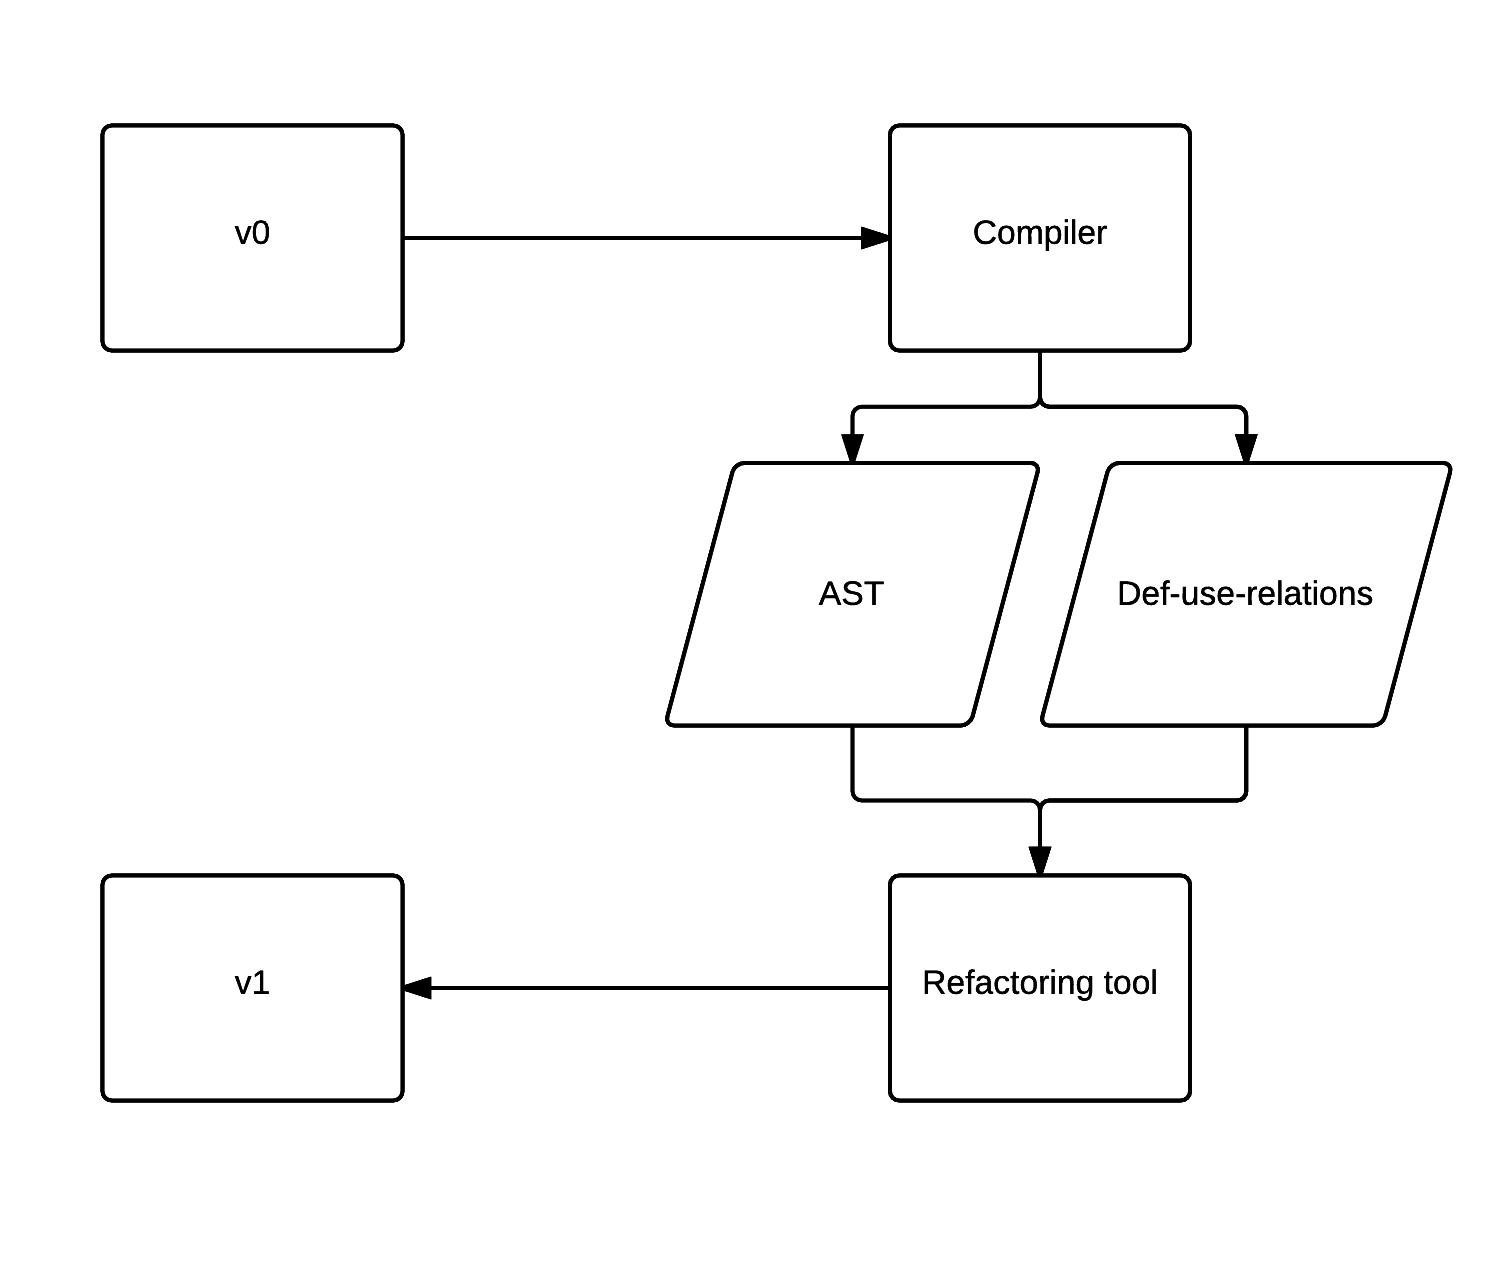
\includegraphics[width=0.95\textwidth]{img/arquitectura.png}
	\caption{Solution's architecture}
	\label{fig:architecture}
\end{figure}


\subsection{Validation}
%In order to evaluate it was implemented a prototype in DrRacket.
In order to validate this architecture some refactoring operations were implemented. 
This allows to validate the architecture and have more trust in this architecture.
To do that it was only validated the refactoring operations that use exclusively the def-use-relations.

\subsubsection{Extract-function}
The user selects the expressions that wants to extract and chooses a name for the new function as seen in {\bf Figure~\ref{fig:extractBefore}}.
Then the user pastes the result of the extraction where he thinks it's the best place for the function. 
The final result can be seen in {\bf Figure~\ref{fig:extractAfter}}.
The extract function refactoring could automatically paste the extracted function, however this way the user can choose the function's location.
\begin{figure}[htbp]
	\centering
	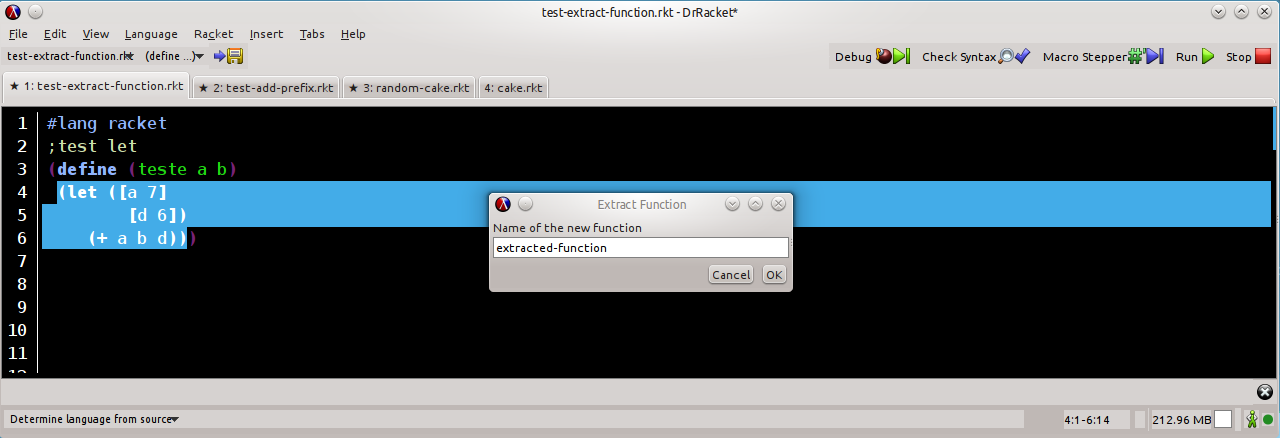
\includegraphics[width=0.95\textwidth]{img/extract1.png}
	\caption{Before the Extract function}
	\label{fig:extractBefore}
\end{figure}

\begin{figure}[htbp]
	\centering
	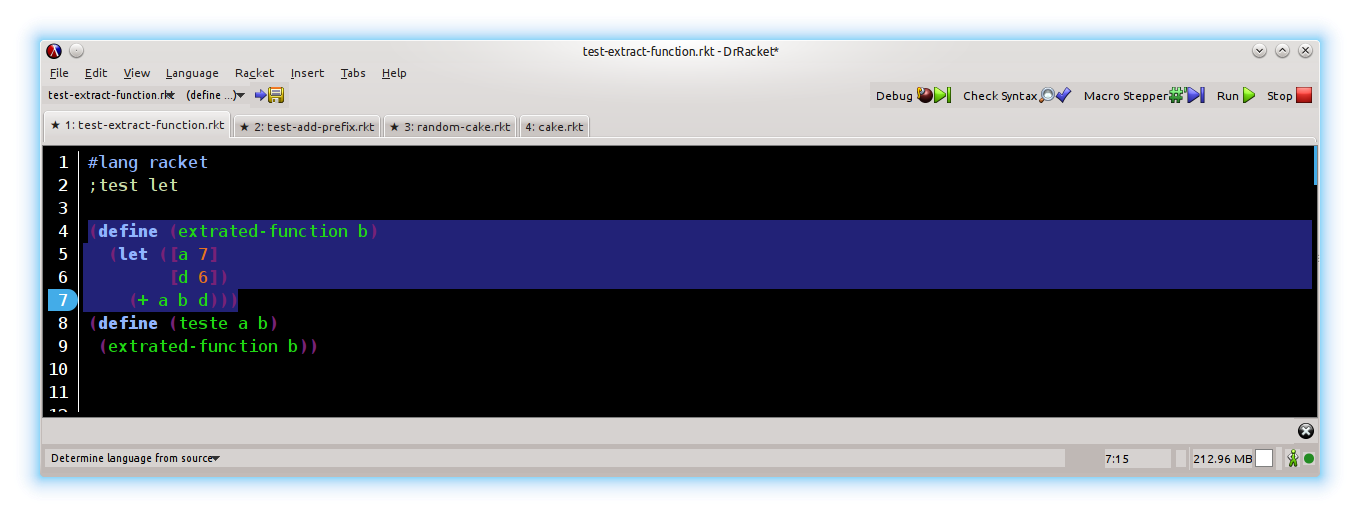
\includegraphics[width=0.95\textwidth]{img/extract2.png}
	\caption{After the Extract function}
	\label{fig:extractAfter}
\end{figure}

\subsubsection{Imported renames}
As explained in ~\ref{ssub:Rename} the DrRacket only refactoring operation, the Rename, has bugs when it has to rename imported functions.
This example regards only when renaming an imported function. 
The user selects the function that wants to be renamed, as seen in {\bf Figure~\ref{fig:renameBefore}} and in this case the user chose ``print-cake'', then the user chooses the new name and the end result is shown in {\bf Figure~\ref{fig:renameAfter}}.
\begin{figure}[htbp]
	\centering
	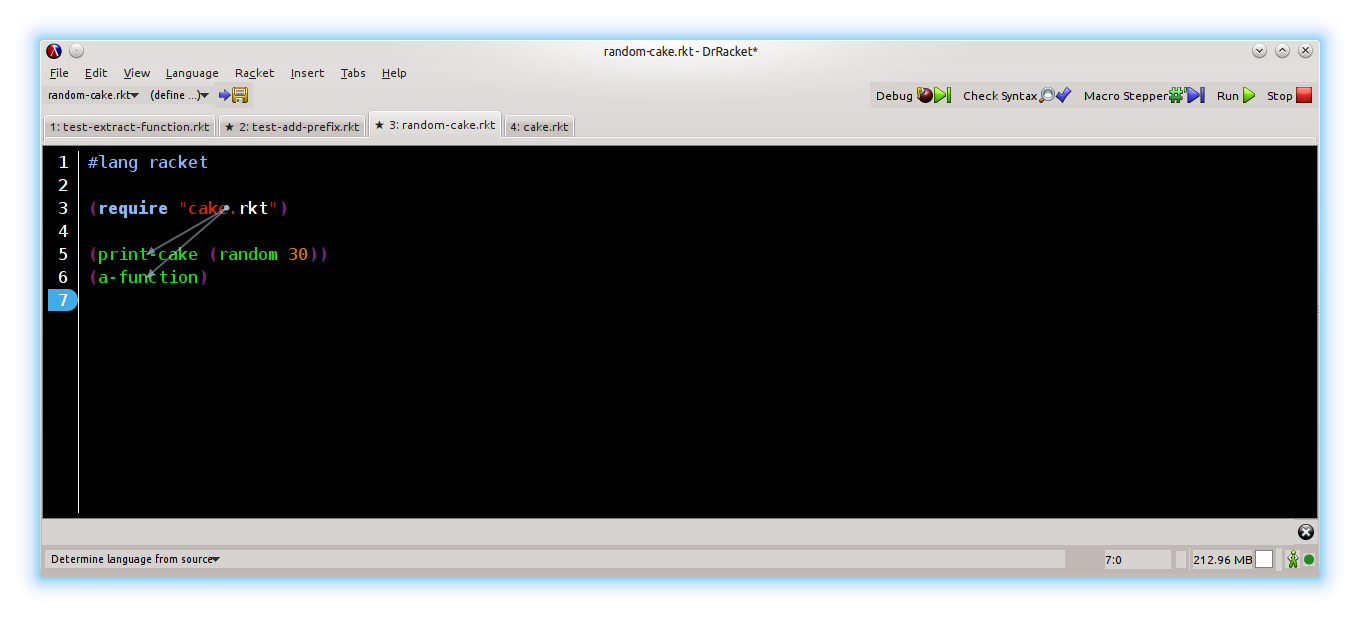
\includegraphics[width=0.95\textwidth]{img/rename1.png}
	\caption{Before the Rename}
	\label{fig:renameBefore}
\end{figure}

\begin{figure}[htbp]
	\centering
	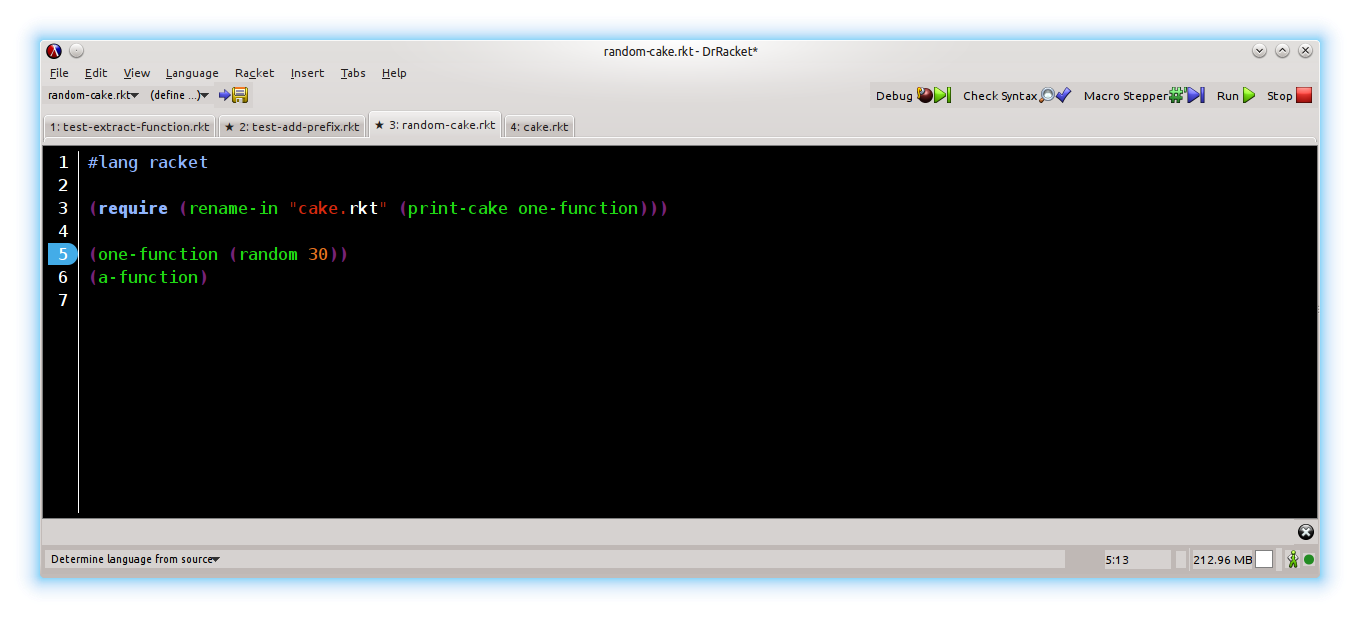
\includegraphics[width=0.95\textwidth]{img/rename2.png}
	\caption{After the Rename}
	\label{fig:renameAfter}
\end{figure}

\subsubsection{Add-prefix}

This is a particular refactoring operation for Racket. Adding a prefix is usually used when there is naming conflicts with two different libraries. The user goes to the library name, and adds a prefix.
In the {\bf Figure~\ref{fig:addPrefixBefore}} the arrows show which functions belong to the ``pict3d'' library.
Then the user selects a name for the prefix that will be added, as shown in {\bf Figure~\ref{fig:addPrefixDuring}}. The final result is shown in {\bf Figure~\ref{fig:addPrefixAfter}}.

\begin{figure}[htbp]
	\centering
	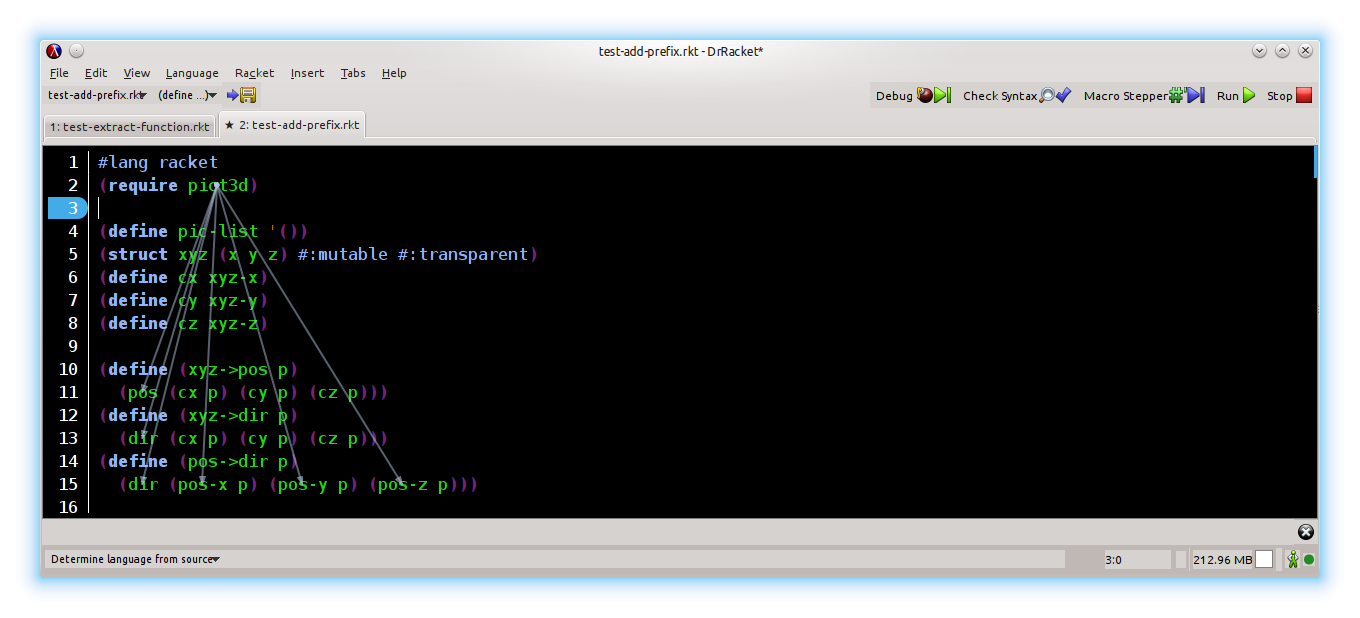
\includegraphics[width=0.95\textwidth]{img/add-prefix.png}
	\caption{Before adding the prefix}
	\label{fig:addPrefixBefore}
\end{figure}

\begin{figure}[htbp]
	\centering
	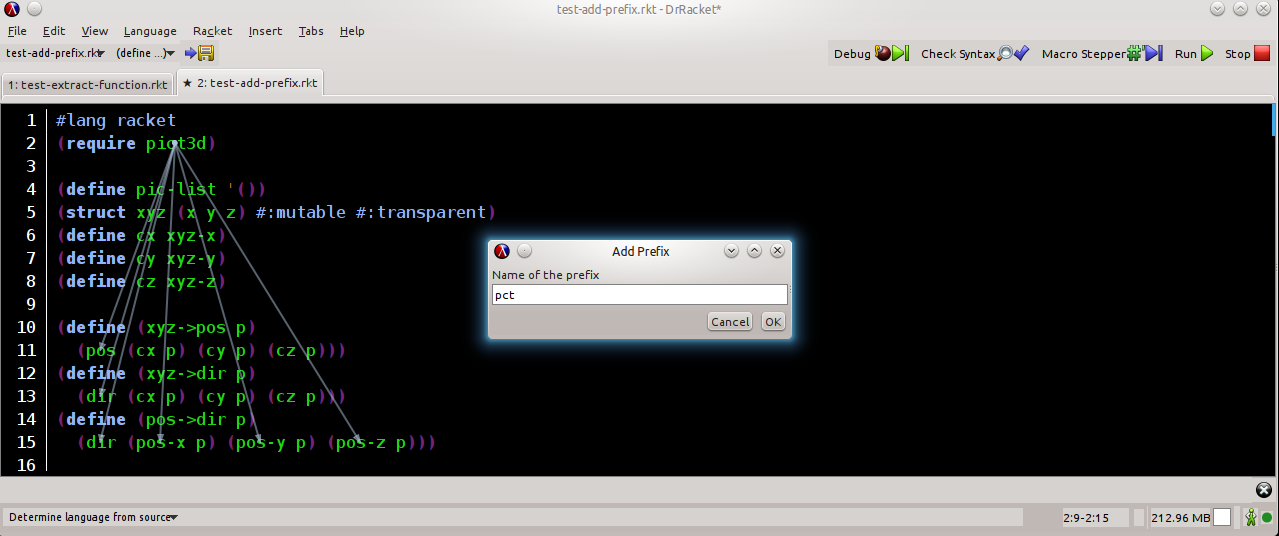
\includegraphics[width=0.95\textwidth]{img/add-prefix1.png}
	\caption{Choosing the prefix}
	\label{fig:addPrefixDuring}
\end{figure}

\begin{figure}[htbp]
	\centering
	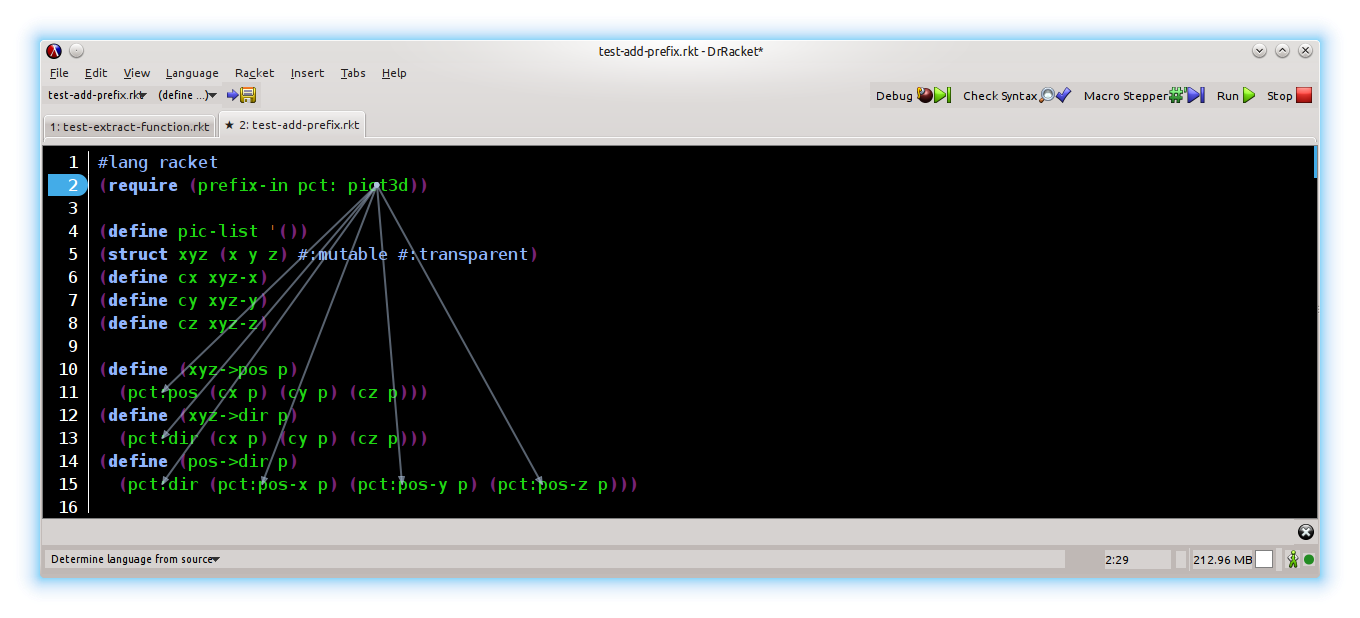
\includegraphics[width=0.95\textwidth]{img/add-prefix2.png}
	\caption{After the Add-prefix refactoring}
	\label{fig:addPrefixAfter}
\end{figure}
%!TEX root = ../report.tex

% 
% Evaluation
% 

\section{Evaluation}

%Explain how you are going to show your results (statistical data, cpu performance etc). Answer the following questions:
%\begin{itemize}
%  \item Why is this solution going to be better than others.
%  \item How am I going to defend that it is better.
%\end{itemize}

In order to evaluate the correctness of the refactoring operations it would be preferable to have a formal proof for each refactoring operation.
However, formal proofs are hard to do and take too much time.
Moreover, formal proofs that exist are usually done for theoretical languages and not for languages actually used, which might explain why even professional refactoring tools such as IntelliJ, Eclipse or NetBeans have errors. \cite{verbaere2006jungl} 
%the formal proofs become useless when a language has introspective actions and has reflexion. even making the alpha conversion possible incorrect if the user lists all the all the variables in the program and renames one it changes the program output. Better example: extracting functions and the program prints all the functions that exists and only uses that functions as input. then it has bugs.

One solution to that problem is to prove correctness informally. 
The proof consists in having several correct Racket programs with unit tests, preferably developed with test-driven-development, then apply some refactoring operations and then run the unit tests again. 
This allows to test if the refactoring operations do not introduce errors in the programs neither change the programs' meaning.

To evaluate the simplicity and usability of the refactoring operations, we will test them by having users following a set of use cases and test the users' response to the tasks.
%!TEX root = ../report.tex

% 
% Conclusions
% 

\section{Conclusions}

%refactoring is used a lot
%BUT tools are underused.
% lack of dynamic refactoring tools and operations when compared with static object oriented ones. some of that exist are dead.
% Intention of creating a tool for unexperienced users to start doing refactoring operations with the tool.


Refactoring operations are important in order to maintain the quality of the software but because they are error prone and time consuming, refactoring tools are needed.
The objective of this overview is to show what exists regarding refactoring tools for dynamic languages and the difference between those tools and tools made for static object oriented languages.

%Although almost every tool made for static object oriented languages has the refactoring operations for 90\% of the refactoring operations used by the users, but in the best case scenario only 27\% of the refactoring operations were tool assisted.

Although almost every tool made for static OBL supports 90\% of the refactoring operations, the users only use refactoring tools for 27\% of the cases. %showing that the major part of the refactoring operations are done manualy]

It also shows how few refactoring operations exist in general for dynamic languages and why it is more difficult to make a refactoring tool for dynamic languages.

In conclusion, this paper shows the importance of having a refactoring tool concerned about the unexperienced users. Besides having dynamic languages as the recommended languages to learn how to program, the dynamic languages are growing. And it might help the users start to use the refactoring tools and refactoring their programs alongside with programming.

%and to show the need of a refactoring tool for dynamic languages targeted for unexperienced programmers





% 
% Bibliography
% 
\bibliographystyle{unsrt} 

% replace example.bib with your .bib
\bibliography{example.bib} 
%\newpage
%!TEX root = ../report.tex

\section{Appendix} % (fold)
\label{sec:attachments}


\end{document}